\documentclass[12pt]{report}
\usepackage[utf8]{inputenc}
\usepackage[russian]{babel}
%\usepackage[14pt]{extsizes}
\usepackage{listings}
\usepackage{graphicx}
\usepackage{amsmath,amsfonts,amssymb,amsthm,mathtools} 
\usepackage{pgfplots}
\usepackage{filecontents}
\usepackage{float}
\usepackage{comment}
\usepackage{indentfirst}
\usepackage{eucal}
\usepackage{enumitem}
%s\documentclass[openany]{book}
\frenchspacing

\usepackage{indentfirst} % Красная строка

\usetikzlibrary{datavisualization}
\usetikzlibrary{datavisualization.formats.functions}

\usepackage{amsmath}


% Для листинга кода:
\lstset{ %
	language=c,                 % выбор языка для подсветки (здесь это С)
	basicstyle=\small\sffamily, % размер и начертание шрифта для подсветки кода
	numbers=left,               % где поставить нумерацию строк (слева\справа)
	numberstyle=\tiny,           % размер шрифта для номеров строк
	stepnumber=1,                   % размер шага между двумя номерами строк
	numbersep=5pt,                % как далеко отстоят номера строк от подсвечиваемого кода
	showspaces=false,            % показывать или нет пробелы специальными отступами
	showstringspaces=false,      % показывать или нет пробелы в строках
	showtabs=false,             % показывать или нет табуляцию в строках
	frame=single,              % рисовать рамку вокруг кода
	tabsize=2,                 % размер табуляции по умолчанию равен 2 пробелам
	captionpos=t,              % позиция заголовка вверху [t] или внизу [b] 
	breaklines=true,           % автоматически переносить строки (да\нет)
	breakatwhitespace=false, % переносить строки только если есть пробел
	escapeinside={\#*}{*)}   % если нужно добавить комментарии в коде
}


\usepackage[left=2cm,right=2cm, top=2cm,bottom=2cm,bindingoffset=0cm]{geometry}
% Для измененных титулов глав:
\usepackage{titlesec, blindtext, color} % подключаем нужные пакеты
\definecolor{gray75}{gray}{0.75} % определяем цвет
\newcommand{\hsp}{\hspace{20pt}} % длина линии в 20pt
% titleformat определяет стиль
\titleformat{\chapter}[hang]{\Huge\bfseries}{\thechapter\hsp\textcolor{gray75}{|}\hsp}{0pt}{\Huge\bfseries}


% plot
\usepackage{pgfplots}
\usepackage{filecontents}
\usetikzlibrary{datavisualization}
\usetikzlibrary{datavisualization.formats.functions}

\begin{document}
	%\def\chaptername{} % убирает "Глава"
	\thispagestyle{empty}
	\begin{titlepage}
		\noindent \begin{minipage}{0.15\textwidth}
			
\includegraphics[width=\linewidth]{img/b_logo}
		\end{minipage}
		\noindent\begin{minipage}{0.9\textwidth}\centering
			\textbf{Министерство науки и высшего образования Российской Федерации}\\
			\textbf{Федеральное государственное бюджетное образовательное учреждение высшего образования}\\
			\textbf{~~~«Московский государственный технический университет имени Н.Э.~Баумана}\\
			\textbf{(национальный исследовательский университет)»}\\
			\textbf{(МГТУ им. Н.Э.~Баумана)}
		\end{minipage}
		
		\noindent\rule{18cm}{3pt}
		\newline\newline
		\noindent ФАКУЛЬТЕТ $\underline{\text{«Информатика и системы управления»}}$ \newline\newline
		\noindent КАФЕДРА $\underline{\text{«Программное обеспечение ЭВМ и информационные технологии»}}$\newline\newline\newline\newline\newline
		
		\begin{center}
			\noindent\begin{minipage}{1.1\textwidth}\centering
				\Large\textbf{  Отчет по лабораторной работе №5}\newline
				\textbf{по дисциплине <<Операционные системы>>}\newline\newline\newline
			\end{minipage}
		\end{center}
		
		\noindent\textbf{Тема} $\underline{\text{Буферизованный и не буферизованный ввод-вывод}}$\newline\newline
		\noindent\textbf{Студент} $\underline{\text{Зайцева А. А.~~~~~~~~~~~~~~~~~~~~}}$\newline\newline
		\noindent\textbf{Группа} $\underline{\text{ИУ7-62Б~~~~~~~~~~~~~~~~~~~~~~~~~~~~}}$\newline\newline
		\noindent\textbf{Оценка (баллы)} $\underline{\text{~~~~~~~~~~~~~~~~~~~~~~~~~~~}}$\newline\newline
		\noindent\textbf{Преподаватель} $\underline{\text{Рязанова Н. Ю.~~~~~~~}}$\newline\newline\newline
		
		\begin{center}
			\vfill
			Москва~---~\the\year
			~г.
		\end{center}
	\end{titlepage}


\chapter*{Структура \_IO\_FILE}

\begin{lstlisting}[language=c, label=_io_file, caption=Листинг структуры \_IO\_FILE]
// /usr/include/x86_64-linux-gnu/bits/types/FILE.h:

#ifndef __FILE_defined
#define __FILE_defined 1

struct _IO_FILE;

/* The opaque type of streams.  This is the definition used elsewhere.  */
typedef struct _IO_FILE FILE;

#endif


// /usr/include/x86_64-linux-gnu/bits/libio.h:
...
struct _IO_FILE {
	int _flags;           /* High-order word is _IO_MAGIC; rest is flags. */
	#define _IO_file_flags _flags
	
	/* The following pointers correspond to the C++ streambuf protocol. */
	/* Note:  Tk uses the _IO_read_ptr and _IO_read_end fields directly. */
	char* _IO_read_ptr;   /* Current read pointer */
	char* _IO_read_end;   /* End of get area. */
	char* _IO_read_base;  /* Start of putback+get area. */
	char* _IO_write_base; /* Start of put area. */
	char* _IO_write_ptr;  /* Current put pointer. */
	char* _IO_write_end;  /* End of put area. */
	char* _IO_buf_base;   /* Start of reserve area. */
	char* _IO_buf_end;    /* End of reserve area. */
	/* The following fields are used to support backing up and undo. */
	char *_IO_save_base; /* Pointer to start of non-current get area. */
	char *_IO_backup_base;  /* Pointer to first valid character of backup area */
	char *_IO_save_end; /* Pointer to end of non-current get area. */
	
	struct _IO_marker *_markers;
	
	struct _IO_FILE *_chain;
	
	int _fileno;
	#if 0
	int _blksize;
	#else
	int _flags2;
	#endif
	_IO_off_t _old_offset; /* This used to be _offset but it's too small.  */
	
	#define __HAVE_COLUMN /* temporary */
	/* 1+column number of pbase(); 0 is unknown. */
	unsigned short _cur_column;
	signed char _vtable_offset;
	char _shortbuf[1];
	
	/*  char* _save_gptr;  char* _save_egptr; */
	
	_IO_lock_t *_lock;
	#ifdef _IO_USE_OLD_IO_FILE
};
...
\end{lstlisting}
	
\chapter{Первая программа}

\begin{lstlisting}[language=c, label=p1, caption=Первая программа]
#include <stdio.h>
#include <fcntl.h>
#include <unistd.h>

int main(void)
{
	// have kernel open connection to file alphabet.txt
    int fd = open("alphabet.txt", O_RDONLY);

	// create two C I/O buffered streams using the above connection 
    FILE *fs1 = fdopen(fd, "r");
    char buff1[20];
    setvbuf(fs1, buff1, _IOFBF, 20);

    FILE *fs2 = fdopen(fd, "r");
    char buff2[20];
    setvbuf(fs2, buff2, _IOFBF, 20);

	// read a char & write it alternatingly from fs1 and fs2
    int flag1 = 1, flag2 = 2;
    while (flag1 == 1 || flag2 == 1)
    {
        char c;

        if ((flag1 = fscanf(fs1, "%c", &c)) == 1)
        {
            fprintf(stdout, "%c", c);
        }

        if ((flag2 = fscanf(fs2, "%c", &c)) == 1)
        {
            fprintf(stdout, "%c", c);
        }
    }
    close(fd);

    return 0;
}
\end{lstlisting}



\begin{figure}[H]
	\centering
	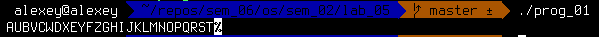
\includegraphics[scale=0.8]{img/prog_01.png}
	\caption{Результат работы первой программы}
	\label{fig:prog_01}
\end{figure}

\begin{lstlisting}[language=c, label=p1thread, caption=Первая программа (реализация с потоками)]
#include <stdio.h>
#include <fcntl.h>
#include <pthread.h>
#include <sys/types.h>
#include <sys/wait.h>
#include <unistd.h>

void *thread_func(void *args)
{
    int flag = 1;
    FILE *fs = (FILE *)args;

    while (flag == 1)
    {
        char c;
        if ((flag = fscanf(fs, "%c", &c)) == 1)
        {
            fprintf(stdout, "Additional thread read: %c\n", c);
        }
    }
}

int main(void)
{
    setbuf(stdout, NULL);

    pthread_t thread;
    int fd = open("alphabet.txt", O_RDONLY);

    FILE *fs1 = fdopen(fd, "r");
    char buff1[20];
    setvbuf(fs1, buff1, _IOFBF, 20);

    FILE *fs2 = fdopen(fd, "r");
    char buff2[20];
    setvbuf(fs2, buff2, _IOFBF, 20);

    if (pthread_create(&thread, NULL, thread_func, (void *)fs2) != 0)
	{
		perror("Error in pthread_create\n");
		return -1;
	}

    int flag = 1;
    while (flag == 1)
    {
        char c;
        if ((flag = fscanf(fs1, "%c", &c)) == 1)
        {
            fprintf(stdout, "Main thread read: %c\n", c);
        }
    }
	// The pthread_join() function suspends processing of the calling thread until the target thread completes.
	// 2 arg - void **status
    pthread_join(thread, NULL);

    close(fd);

    return 0;
}
\end{lstlisting}


\begin{figure}[H]
	\centering
	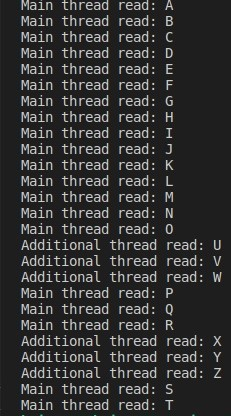
\includegraphics[scale=0.6]{img/prog_01_thread.png}
	\caption{Результат работы первой программы (с потоками)}
	\label{fig:prog_01_thread}
\end{figure}



\begin{figure}[H]
	\centering
	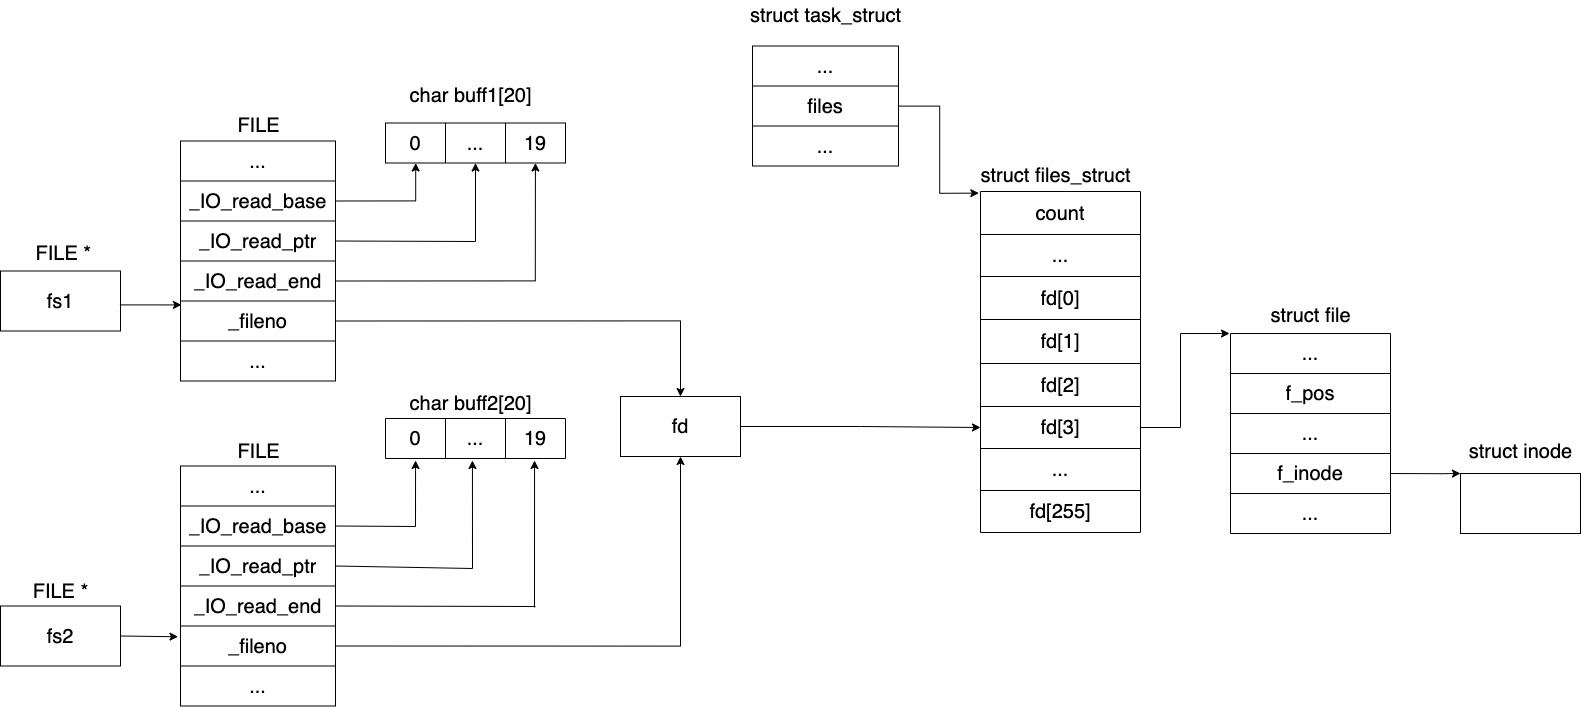
\includegraphics[scale=0.33]{img/prog_01_schema.jpg}
	\caption{Схема структур, используемых в первой программе}
	\label{fig:prog_01_schema}
\end{figure}

Системный вызов open() создает новый файловый дескриптор для открытого только для чтения файла "alphabet.txt" (который содержит символы Abcdefghijklmnopqrstuvwxyz), создавая запись в системной таблице открытых файлов. Эта запись регистрирует смещение в файле и флаги состояния файла. Дескриптор файла является ссылкой на одну из этих записей. 

Вызов fdopen() возвращает указатель на структуру типа FILE (fs1 и fs2), которая ссылается на дескриптор открытого файла, созданный ранее. 
	
Вызов функции setvbuf() (для fs1 и fs2)  явно задает буффер и его размер (20 байт) и меняет тип буферизации на полную (\_IOFBF).

При первом вызове fscanf()  (для fs1) буффер buff1 полностью заполнится первыми 20 символами. Значение f\_pos в структуре struct\_file открытого файла увеличится на 20. При следующем вызове fscanf() (для fs2) в buff2 считаются оставшиеся 6 символов, начиная с f\_pos (fs1 и fs2 ссылаются на один и тот же дескриптор fd).


Затем в однопоточной программе в цикле поочередно выводятся символы из buff1 и buff2 (так как в buff2 записались лишь оставшиеся 6 символов, после 6 итерации цикла будут выводится символы только из buff1). В двупоточной программе же (в данном запуске) главный поток начал в цикле выводить символы из своего буффера, затем потерял квант,??




\chapter{Вторая программа}

\begin{lstlisting}[language=c, label=p2, caption=Вторая программа]
#include <fcntl.h>
#include <unistd.h>

int main(void)
{
    int fd1 = open("alphabet.txt", O_RDONLY);
    int fd2 = open("alphabet.txt", O_RDONLY);
    int rc1 = 1, rc2 = 1;

    while (rc1 == 1 && rc2 == 1)
    {
        char c;

        rc1 = read(fd1, &c, 1);
        if (rc1 == 1)
        {
            write(1, &c, 1);

            rc2 = read(fd2, &c, 1);
            if (rc2 == 1)
            {
                write(1, &c, 1);
            }
        }
    }
    close(fd1);
    close(fd2);


    return 0;
}
\end{lstlisting}

\begin{figure}[H]
	\centering
	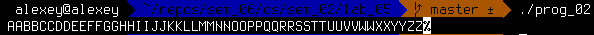
\includegraphics[scale=0.9]{img/prog_02.png}
	\caption{Результат работы второй программы}
	\label{fig:prog_02}
\end{figure}




\begin{lstlisting}[language=c, label=p2thread, caption=Вторая программа (с потоками)]
#include <stdio.h>
#include <fcntl.h>
#include <unistd.h>
#include <pthread.h>

void *thread_func(void *args)
{
    int fd2 = open("alphabet.txt", O_RDONLY);
    int rc = 1;

    while (rc == 1)
    {
        char c;
        rc = read(fd2, &c, 1);
        if (rc == 1)
        {
            write(1, &c, 1);
        }
    }
    close(fd2);
}

int main(void)
{
    int fd1 = open("alphabet.txt", O_RDONLY);
    

    pthread_t thread;

    if (pthread_create(&thread, NULL, thread_func, 0) != 0)
	{
		perror("error in pthread_create\n");
		return -1;
	}

    int rc = 1;

    while (rc == 1)
    {
        char c;
        rc = read(fd1, &c, 1);
        if (rc == 1)
        {
            write(1, &c, 1);
        }
    }

    pthread_join(thread, NULL);
    close(fd1);

    return 0;
}

\end{lstlisting}



\begin{figure}[H]
	\centering
	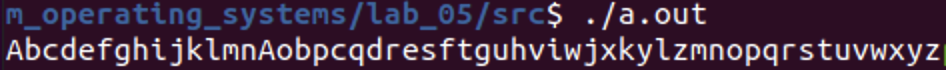
\includegraphics[scale=1]{img/prog_02_thread.png}
	\caption{Результат работы второй программы (с потоками)}
	\label{fig:prog_02_thread}
\end{figure}


\begin{figure}[H]
	\centering
	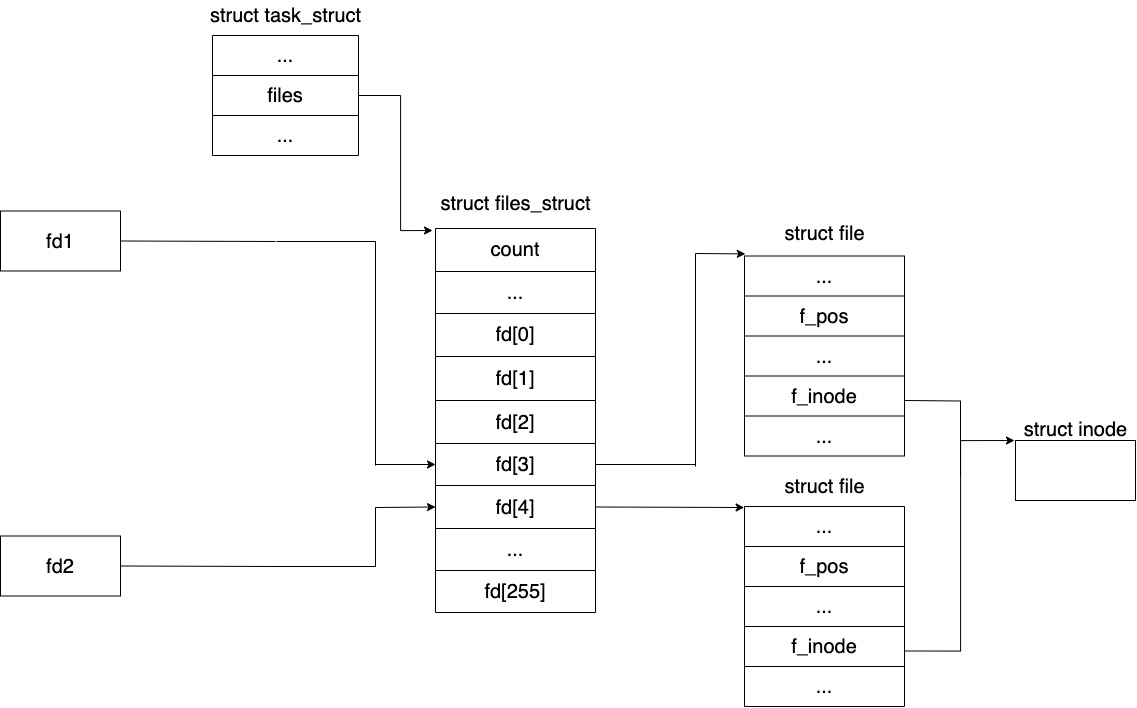
\includegraphics[scale=0.4]{img/prog_02_schema.jpg}
	\caption{Схема структур второй программы}
	\label{fig:prog_02_schema}
\end{figure}


Два системных вызова open() создают два новых файловых дескриптора для открытого только для чтения файла, создавая две записи в системной таблице открытых файлов. Каждая запись регистрирует смещение в файле и флаги состояния файла. 

Таким образом, в программе существует две различные структуры struct file, которые при этом ссылаются на одну и ту же структуру struct inode. В каждой структуре свое поле f\_pos (то есть смещения независимы), поэтому на экран каждый символ выводится дважды.

При этом в однопоточной программе в цикле каждый символ из файла выводится два раза подряд, а в двупоточной заранее предсказать порядок вывода символов невозможно, так как потоки выполняются параллельно (при этом дочерний поток начинает вывод позже, так как затрачивается время на его создание).






\chapter{Третья программа}

\textbf{На рис. \ref{fig:prog_03_schema} представлена схема структур, используемых в третьей программе.}

\begin{figure}[H]
	\centering
	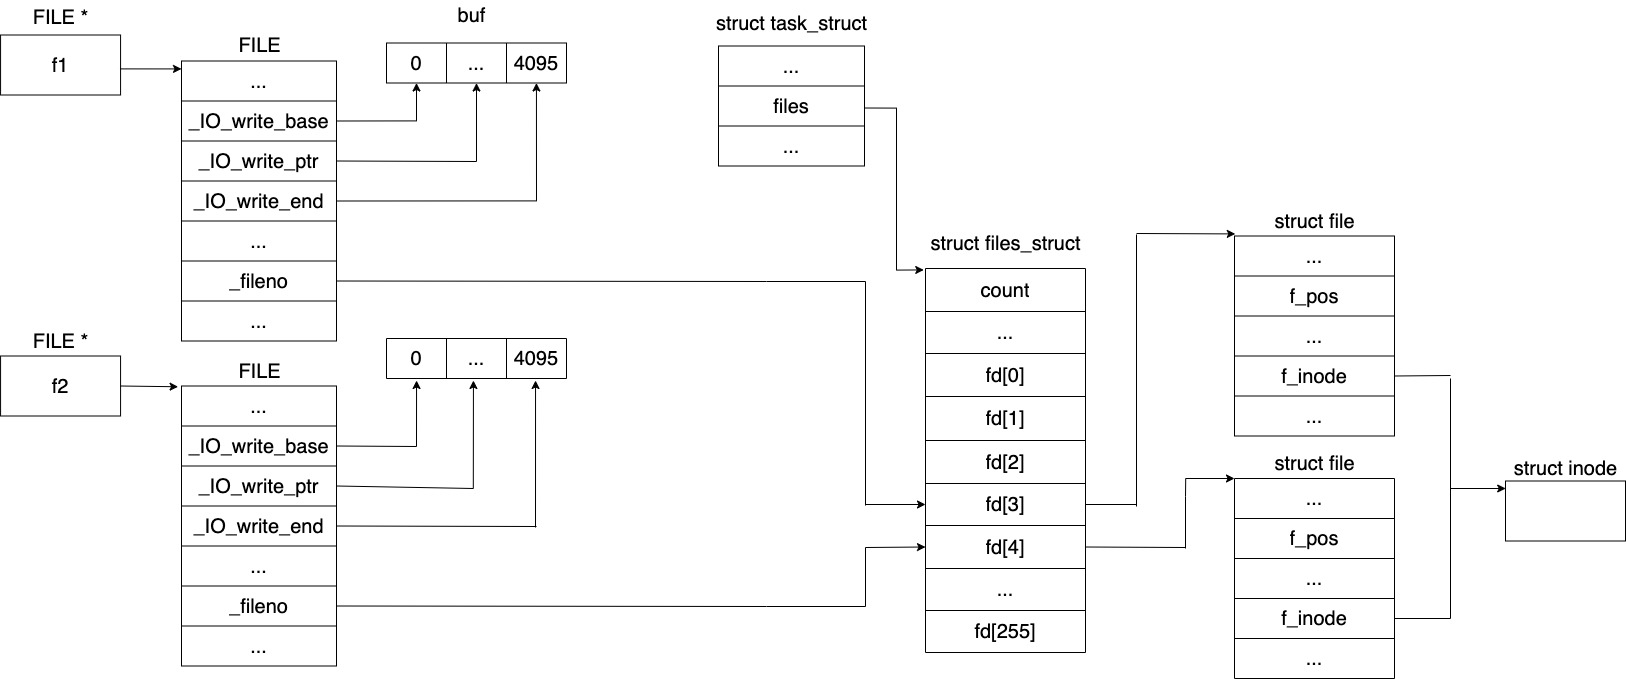
\includegraphics[scale=0.32]{img/prog_03_schema.jpg}
	\caption{Схема структур программы №2}
	\label{fig:prog_03_schema}
\end{figure}

\begin{itemize}
	\item Файл открывается на запись два раза, с помощью функции \texttt{fopen()};
	\item функция \texttt{fprintf()} предоставляет буферизованный вывод - буфер создается без нашего вмешательства;g
	\item изначально информация пишется в буфер, а из буфера в файл если произошло одно из событий:
		\subitem буффер полон;
		\subitem вызвана функция \texttt{fclose()};
		\subitem вызвана функция \texttt{fflush()};
	\item в случае нашей программы, информация в файл запишется в результате вызова функция \texttt{fclose()};
	\item из-за того \texttt{f\_pos} независимы для каждого дескриптора файла, запись в файл будет производится с самого начала;
	\item таким образом, информация записаная при первом вызове \texttt{fclose()} будет потеряна в результате второго вызова \texttt{fclose()} (см. рис. \ref{fig:prog_03}).
	\item в многопоточной реализации результат аналогичен - с помощью \texttt{pthread\_join} мы дожидаемся вызова \texttt{fclose()} для \texttt{f2} в отдельном потоке и далее вызываем \texttt{fclose()} для \texttt{f1}.
\end{itemize}

\begin{lstlisting}[language=c, label=p3, caption=Программа №3]
#include <stdio.h>
#include <fcntl.h>
#include <unistd.h>
#define OK 0
#define FILE_NAME "data/out.txt"
#define SPEC "%c"

int main()
{
	FILE *f1 = fopen(FILE_NAME, "w");
	FILE *f2 = fopen(FILE_NAME, "w");
	
	for (char c = 'a'; c <= 'z'; c++)
	{
		if (c % 2)
		{
			fprintf(f1, SPEC, c);
		}
		else
		{
			fprintf(f2, SPEC, c);
		}
	}
	
	fclose(f2);
	fclose(f1);
	return OK;
}
\end{lstlisting}

""\newline
\textbf{На рис. \ref{fig:prog_03} представлен результат работы третьей программы.}

\begin{figure}[H]
	\centering
	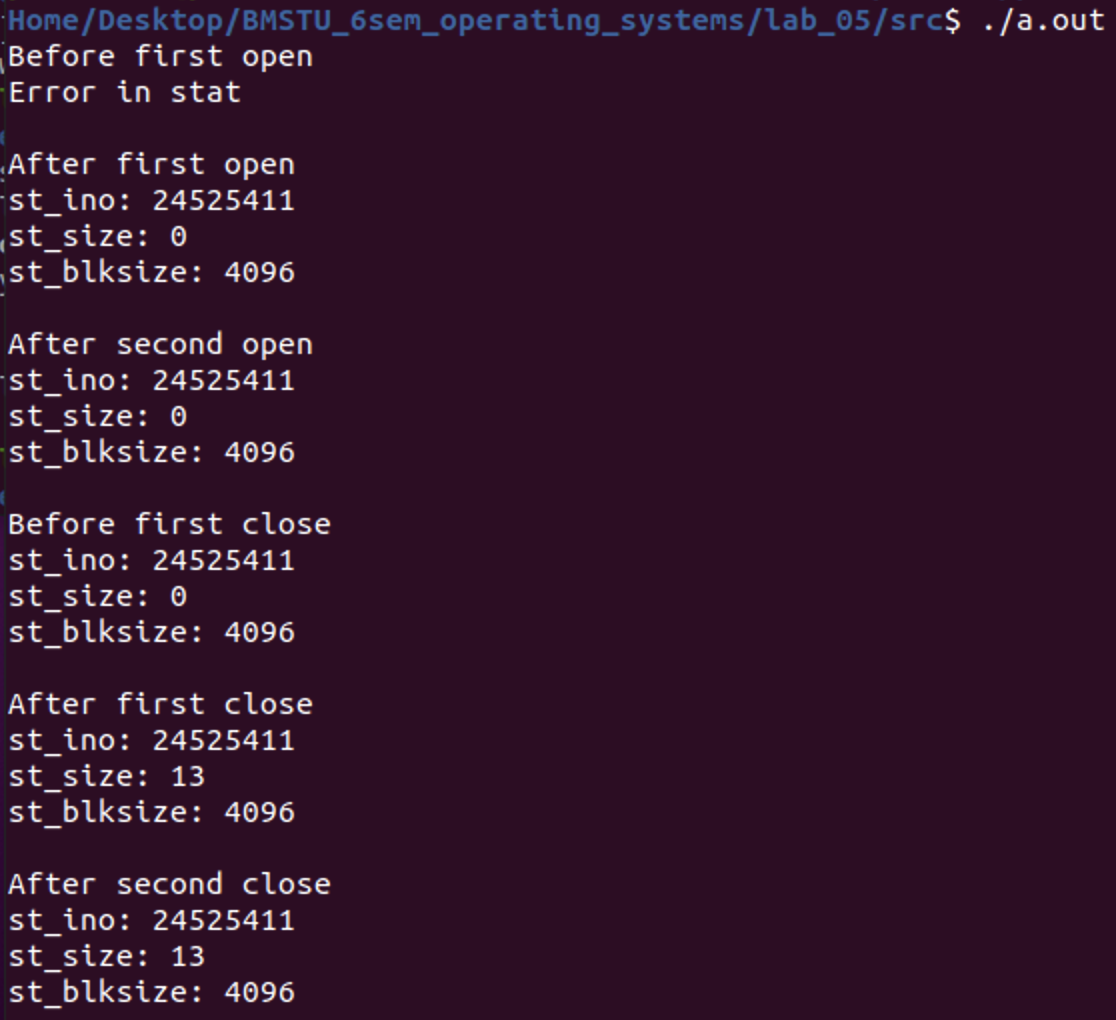
\includegraphics[scale=0.8]{img/prog_03.png}
	\caption{Результат работы третьей программы}
	\label{fig:prog_03}
\end{figure}

\begin{lstlisting}[language=c, label=p3thread, caption=Программа №3 (реализация с потоками)]
#include <stdio.h>
#include <fcntl.h>
#include <pthread.h>
#include <unistd.h>
#define OK 0
#define FILE_NAME "data/out.txt"
#define SPEC "%c"

void *run_buffer(void *args)
{
	FILE *f = (FILE *)args;
	
	for (char c = 'b'; c <= 'z'; c += 2)
	{
		fprintf(f, SPEC, c);
	}
	
	fclose(f);
	return NULL;
}

int main()
{
	FILE *f1 = fopen(FILE_NAME, "w");
	FILE *f2 = fopen(FILE_NAME, "w");
	
	pthread_t thread;
	int rc = pthread_create(&thread, NULL, run_buffer, (void *)(f2));
	
	for (char c = 'a'; c <= 'z'; c += 2)
	{
		fprintf(f1, SPEC, c);
	}
	
	pthread_join(thread, NULL);
	fclose(f1);
	return OK;
}
\end{lstlisting}

""\newline
\textbf{На рис. \ref{fig:prog_03_thread} представлен результат работы второй программы (с потоками).}

\begin{figure}[H]
	\centering
	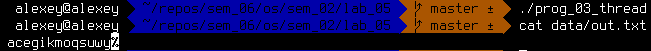
\includegraphics[scale=0.8]{img/prog_03_thread.png}
	\caption{Результат работы третьей программы (с потоками)}
	\label{fig:prog_03_thread}
\end{figure}

\bibliographystyle{utf8gost705u}  % стилевой файл для оформления по ГОСТу
\bibliography{51-biblio}          % имя библиографической базы (bib-файла)
	
\end{document}
